%% ------------------------------------------------------------------------- %%
\chapter{Experimento}
\label{cap:experimento}

Neste capítulo apresentamos os resultados da avaliação do uso das redes convolucionais no problema de \textit{code retrieval}. Utilizamos a nossa arquitetura proposta no Capítulo~\ref{cap:abordagem}. E para comparar, utilizamos duas arquiteturas: uma arquitetura de referência \textit{Embedding} e outra arquitetura que é o estado da arte em recuperação de trecho de código-fonte proposta por \cite{cambronero-deep-learning-code-search:2019}. Os resultados da arquitetura CNN foram promissores. A arquitetura apresentou um valor de métrica \acrfull{mrr} de $0,58$. \todo{atualizar o valor} Em $75\%$ das vezes, as respostas corretas apareceram entre as 3 primeiras posições, de um total de 50 possíveis respostas. \todo{atualizar o valor}

\section{Conjunto de dados}
\label{sec:conjunto-dados}

Para este estudo, utilizamos parte do conjunto de dados disponibilizados por \cite{yao-2018}. Esse conjunto é formado por $\bm{147.546}$ pares de questões em inglês e trechos de código-fonte em Python e $\bm{119.519}$ em SQL. Estes pares foram coletados do site \Gls{sof} e disponibilizados publicamente através de um repositório no \Gls{github} pelos pesquisadores\footnote{\url{https://github.com/LittleYUYU/StackOverflow-Question-Code-Dataset}}. Uma peculiaridade desses dados em relação aos dados utilizados nos outros trabalhos \cite{iyer-etal-2016-summarizing, Allamanis-bimodal-source-code-natural-language:2015}, é o fato de conter questões do tipo \textit{how-to-do-it}. As respostas para este tipo de questão costumam ser mais diretas e ter apenas um trecho de código-fonte como solução \citep{yao-2018}. Essas questões normalmente expressam as intenções do desenvolvedor, indo ao encontro com a nossa definição da Seção~\ref{sec:code-retrieval-definicao} adotada para o problema de \textit{code retrieval}.

Os dados disponibilizados por \cite{yao-2018} são divididos em 3 (três) subconjuntos distintos. Um subconjunto é formado apenas por questões coletadas do \Gls{sof} que continham apenas um trecho de código-fonte na descrição da resposta. O outro é formado por questões que apresentavam mais de um trecho de código-fonte na descrição. O terceiro é formado por pares de questões e trechos de código-fonte anotados manualmente. A divisão dos subconjuntos de amostras de pares de questões e trechos de código podem ser visualizados na Figura~\ref{fig:distinct-subset-python-pair-question-code}.

\begin{figure}[h]
\centering
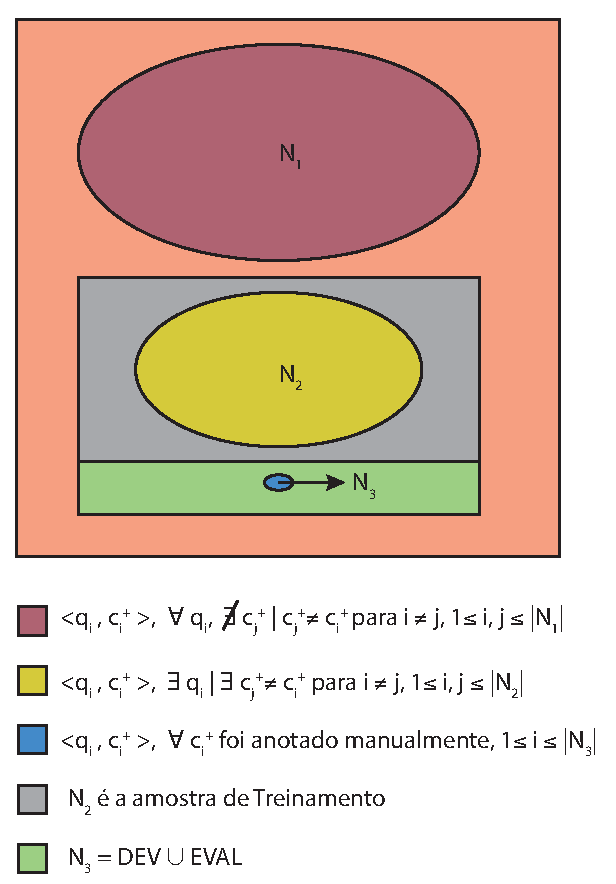
\includegraphics[width=0.6\textwidth]{figuras/cap-experimento/distinct-subsets-yao-sample.pdf}
\caption{Divisão das amostras de pares de questões e trechos de código disponibilizados por \cite{yao-2018}: $N_{1} = \{(q_{i}, c_{i}^{+})\;,\; \forall\; q_{i},\;\nexists\; c_{j}^{+}\; |\; c_{j}^{+} \neq c_{i}^{+}\; \text{para}\; i \neq j,\; 1 \leq i,j \leq |N_{1}| \}$, $N_{2} = \{(q_{i}, c_{i}^{+})\;,\; \exists\; q_{i}\; | \;\exists\; c_{j}^{+} \neq c_{i}^{+}\; \text{para} \; i \neq j,\; 1 \leq i,j \leq |N_{2}| \}$, $N_{3} = \{(q_{i}, c_{i}^{+}),\; \forall\; c_{i}^{+} \text{foi anotado manualmente}, 1 \leq i \leq |N_{3}| \}$. Onde $N_{1} \cap N_{2} \cap N_{3} = \varnothing$, $q_{i} \in \mathbb{Q}$ e $c_{i}^{+},  c_{j}^{+} \in \mathbb{C}$. E $c_{i}^{+}, c_{j}^{+}$ são respostas anotadas como corretas. $\mathbb{Q}$ e $\mathbb{C}$ representam o conjunto de questões e trechos de código respectivamente.} 
\label{fig:distinct-subset-python-pair-question-code}
\end{figure}

Nos casos em que há mais de um trecho de código-fonte na descrição da resposta, um trecho de código não é necessariamente uma solução para a pergunta. No exemplo a seguir, os trechos \emph{T2} e \emph{T4} não são soluções para a questão. Já o trecho \emph{T2} apenas inicializa um array e o trecho \emph{T4} mostra a saída do comando \textit{print} para o vetor já convertido\footnote{Site: \url{https://stackoverflow.com/questions/34349762/convert-2d-numpy-array-to-string} Esta questão apresenta 6 trechos de código-fonte, mas para melhor visualização, optamos por colocar apenas 4 trechos em nosso exemplo\label{foot:exemplo-stackoverflow-mais-de-um-trecho}}.



\begin{tcolorbox}[colframe=orange!75!black,colback=gray!15!white,fonttitle=\bfseries,adjusted title=\large{Título da questão: convert 2d numpy array to string}~\ref{foot:exemplo-stackoverflow-mais-de-um-trecho}]
\begin{mypythongreen}{Trecho T1: A one-liner will do:}
b = '\n'.join('\t'.join('%0.3f' %x for x in y) for y in a)
\end{mypythongreen}

\begin{mypythonred}{Trecho T2: Using a simpler example:}
>>> a = np.arange(25, dtype=float).reshape(5, 5)
>>> a
array([[  0.,   1.,   2.,   3.,   4.],
       [  5.,   6.,   7.,   8.,   9.],
       [ 10.,  11.,  12.,  13.,  14.],
       [ 15.,  16.,  17.,  18.,  19.],
       [ 20.,  21.,  22.,  23.,  24.]])
\end{mypythonred}
\begin{mypythongreen}{Trecho T3: is equivalent to:}
res = []
for y in a:
    res.append('\t'.join('%0.3f' %x for x in y))
b = '\n'.join(res)
\end{mypythongreen}
\begin{mypythonred}{Trecho T4: prints this:}
0.000   1.000   2.000   3.000   4.000
5.000   6.000   7.000   8.000   9.000
10.000  11.000  12.000  13.000  14.000
15.000  16.000  17.000  18.000  19.000
20.000  21.000  22.000  23.000  24.000
\end{mypythonred}
\end{tcolorbox}






Para diferenciar estes casos, \cite{yao-2018} anotaram os pares com $\bm{1}$, quando o trecho é solução para a pergunta e $\bm{0}$, em caso contrário. Esta anotação foi feita automaticamente por um framework proposto por \cite{yao-2018}. Ao final, o conjunto de dados é dividido da seguinte maneira:

\begin{table}[h]
\centering
\begin{tabular}{ p{16em} P{10em} P{10em} }
\hline
  & \multicolumn{2}{c}{\textbf{Questão}}\\
\hline
\textbf{Código-fonte} & \textbf{Python} & \textbf{SQL}  \\
\hline

$N_{1}$: Apenas 1 trecho de código na descrição da resposta & $85.294$ & $75.637$ \\

$N_{2}$: Trechos de código-fonte anotados automaticamente & $60.083$ & $41.826$ \\

$N_{3}$: Trechos de código-fonte anotados manualmente & $2.169$ & $2.056$  \\

 \hline
 \textbf{Total} & $\bm{147.546}$ & $\bm{119.519}$\\
 \hline 
 
\end{tabular}
\caption{Divisão do conjunto de dados disponibilizado por \cite{yao-2018}. O conjunto formado por "Trechos de código-fonte anotados automaticamente" contém questões que tem mais de um trecho de código-fonte por resposta. Quando há mais de um trecho de código-fonte por resposta, nem todo trecho é uma solução. Neste caso, \cite{yao-2018} criaram um framework para anotá-los automaticamente. Eles obtiveram F1 de $0,916$ e acurácia de $0,911$ em seus testes de classificação automática das respostas corretas.}
\label{table:summary-training-data-yao-staqc}
\end{table}

\section{Treinamento e avaliação}
\label{sec:treinamento-avaliacao}

Para o treinamento e avaliação do modelo, utilizamos apenas os pares de questões e trechos de código-fonte em Python. Utilizamos os conjuntos $N_{2}$ e $N_{3}$ conforme a Figura~\ref{fig:distinct-subset-python-pair-question-code}. O conjunto de amostras $N_{2}$ apresenta uma variabilidade maior, em torno de 27\% das questões contém mais de um trecho de código-fonte anotados como correto, i.e., 27\% das perguntas tem mais de uma opção de solução.

Quanto ao ... Adotamos o mesmo procedimento de treinamento e avaliação proposto por \cite{iyer-etal-2016-summarizing}. Para o treinamento, foi utilizado o conjunto com $60.083$ pares. E durante o treinamento de 6000 .... 18000 foram para.... Para escolha do modelo e avaliação final, foi utilizado o conjunto de dados anotados manualmente. A divisão das amostras para treinamento e avaliação podem ser visualizadas na Tabela~\ref{table:divisao-amostras}. 

\begin{table}[h]
\centering
\begin{tabular}{ p{3cm} r  }
 \hline
 \textbf{Amostras} & \textbf{Quantidade de pares $<q_{i}, c_{i}^{+}>$}\\
 \hline
 Treinamento & $60.083$\\
 
 DEV & $1.085$ \\
 
 EVAL & $1.084$\\
 \hline
 \textbf{Total} & $\bm{62.252}$\\
 \hline
\end{tabular}
\caption{Divisão das amostras para treinamento e avaliação. O conjunto de dados é formado por pares $<q_{i}, c_{i}^{+}>$, onde $q_{i}$ é uma questão e $c_{i}^{+}$ é um trecho de código-fonte anotado como correto. O conjunto formado por pares anotados manualmente foi dividido em DEV e EVAL conforme o procedimento descrito por \cite{iyer-etal-2016-summarizing}. É possível visualizar uma ilustração deste procedimento nas Figuras \ref{fig:evaluation-process} e \ref{fig:final-evaluation-process}.}
\label{table:divisao-amostras}
\end{table}

De acordo com a Tabela~\ref{table:statistical-descriptive-of-pythons-sample}, as questões tem aproximadamente em média $9$ palavras com um desvio padrão de $\pm 3.71$. Já os trechos de código apresentam aproximadamente uma média de $44$ e um desvio padrão de $\pm 49$. O valor alto do desvio padrão para os trechos de código é um indicativo de maior variabilidade da quantidade de palavras. Este valor da média e desvio padrão são influenciados também por pontos fora da curva, i.e., trechos de código com uma enorme quantidade de palavras. Então, para entender melhor como está distribuída esta quantidade, apresentamos os percentis na Tabela~\ref{table:statistical-descriptive-of-pythons-sample} e o diagrama de caixa com os respectivos quartis na Figura~\ref{fig:boxplot-number-of-words}.

Tanto pela Tabela~\ref{table:statistical-descriptive-of-pythons-sample} quanto pela Figura~\ref{fig:boxplot-number-of-words}, podemos verificar que as questões apresentam um variabilidade e quantidade menor de palavras. Aproximadamente 50\% das questões tem em torno de $6$ a $11$ palavras. Enquanto os trechos de código apresentam 50\% das vezes a quantidade aproximada de $15$ a $54$ palavras. A partir destas informações, podemos dizer que a recuperação de trecho de código-fonte, no nosso caso, é constituída por questões relativamente curtas e trechos de código que variam de 1 (uma) a 3 (três) sentenças de tamanho em linguagem natural \citep{casi-newell-sentence-length-2018}. 




\begin{table}[h]
\centering
\begin{tabular}{ p{5em} P{4em} P{4em} P{4em} P{4em} P{4em} P{4em} }
\hline
  & \multicolumn{5}{c}{\textbf{Quantidade de palavras}}\\
\hline
 & \textbf{$\mathbf{N_{2}}$\_Q} & \textbf{$\mathbf{N_{2}}$\_C} & \textbf{Dev\_Q} & \textbf{Dev\_C} & \textbf{Eval\_Q} & \textbf{Eval\_C}  \\
\hline

Média &	 $8.89$ & $44.41$ &	 $9.15$ & $44.31$ &	 $9.35$ & $42.78$ \\

Desvio padrão & $3.65$ & $55.19$ &	 $3.64$ & $51.87$ &	 $3.85$ & $43.82$ \\

Mínimo & $2$ & $1$ &	 $3$ & $1$ &	 $3$ & $2$ \\ 

25\% & $6$ & $16$ &	 $7$ & $15$ &	 $6$ & $15$ \\

50\% & $8$ & $30$ &	 $9$ & $29$ &	 $9$ & $29$ \\

75\% & $11$ & $54$ &	 $11$ & $52$ &	 $11$ & $55$ \\

Máximo & $32$ & $3566$ &	 $25$ & $708$ &	 $27$ & $439$ \\
 
 
 \hline 
 
\end{tabular}
\caption{Estatística descritiva da amostra de questões e trechos de código em Python utilizados no treinamento e avaliação dos modelos. O prefixo $\mathbf{N_{2}}$ refere-se a amostra de treinamento, conforme a Figura~\ref{fig:distinct-subset-python-pair-question-code}. Os prefixos \textbf{Dev} e \textbf{Eval} referem-se a amostra para escolha do modelo e a amostra para avaliação final conforme procedimento ilustrado nas Figuras \ref{fig:evaluation-process} e \ref{fig:final-evaluation-process}. Os sufixos \textbf{Q} e \textbf{C} referem-se ao conjunto de palavras das questões e trechos de código-fonte respectivamente. Esta tabela inclui a média, desvio padrão e os percentis 25\%, 50\% e 75\% após o pré-processamento. Os detalhes sobre o pré-processamento estão presentes na Seção~\ref{sec:pre-processamento}.}
\label{table:statistical-descriptive-of-pythons-sample}
\end{table}

\begin{figure}[h]
\centering
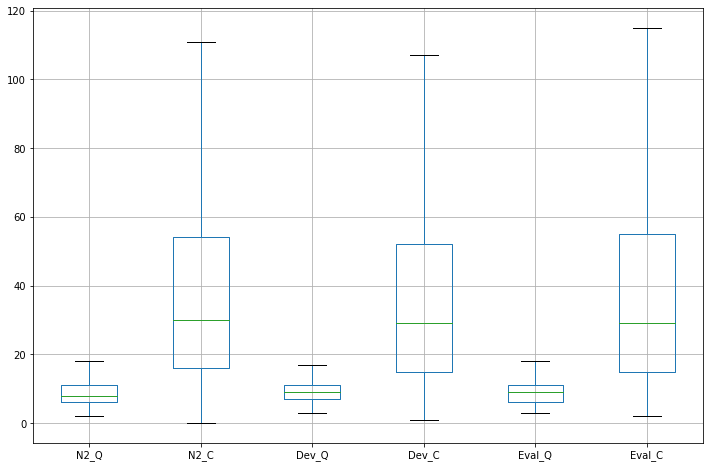
\includegraphics[width=1\textwidth]{figuras/cap-experimento/boxplot_number_of_words.png}
\caption{Diagrama de caixa para visualizar graficamente a distribuição da quantidade de palavras das questões e trechos de código-fonte por meio de quartis. Este diagrama de caixa exibe o Q1 (primeiro quartil), Q2 (segundo quartil) e Q3 (terceiro quartil). Eles referem-se aos percentis 25\%, 50\% e 75\% da Tabela~\ref{table:statistical-descriptive-of-pythons-sample}. O segundo quartil (Q2) refere-se a mediana. }. 
\label{fig:boxplot-number-of-words}
\end{figure}


\begin{figure}[h]
\centering
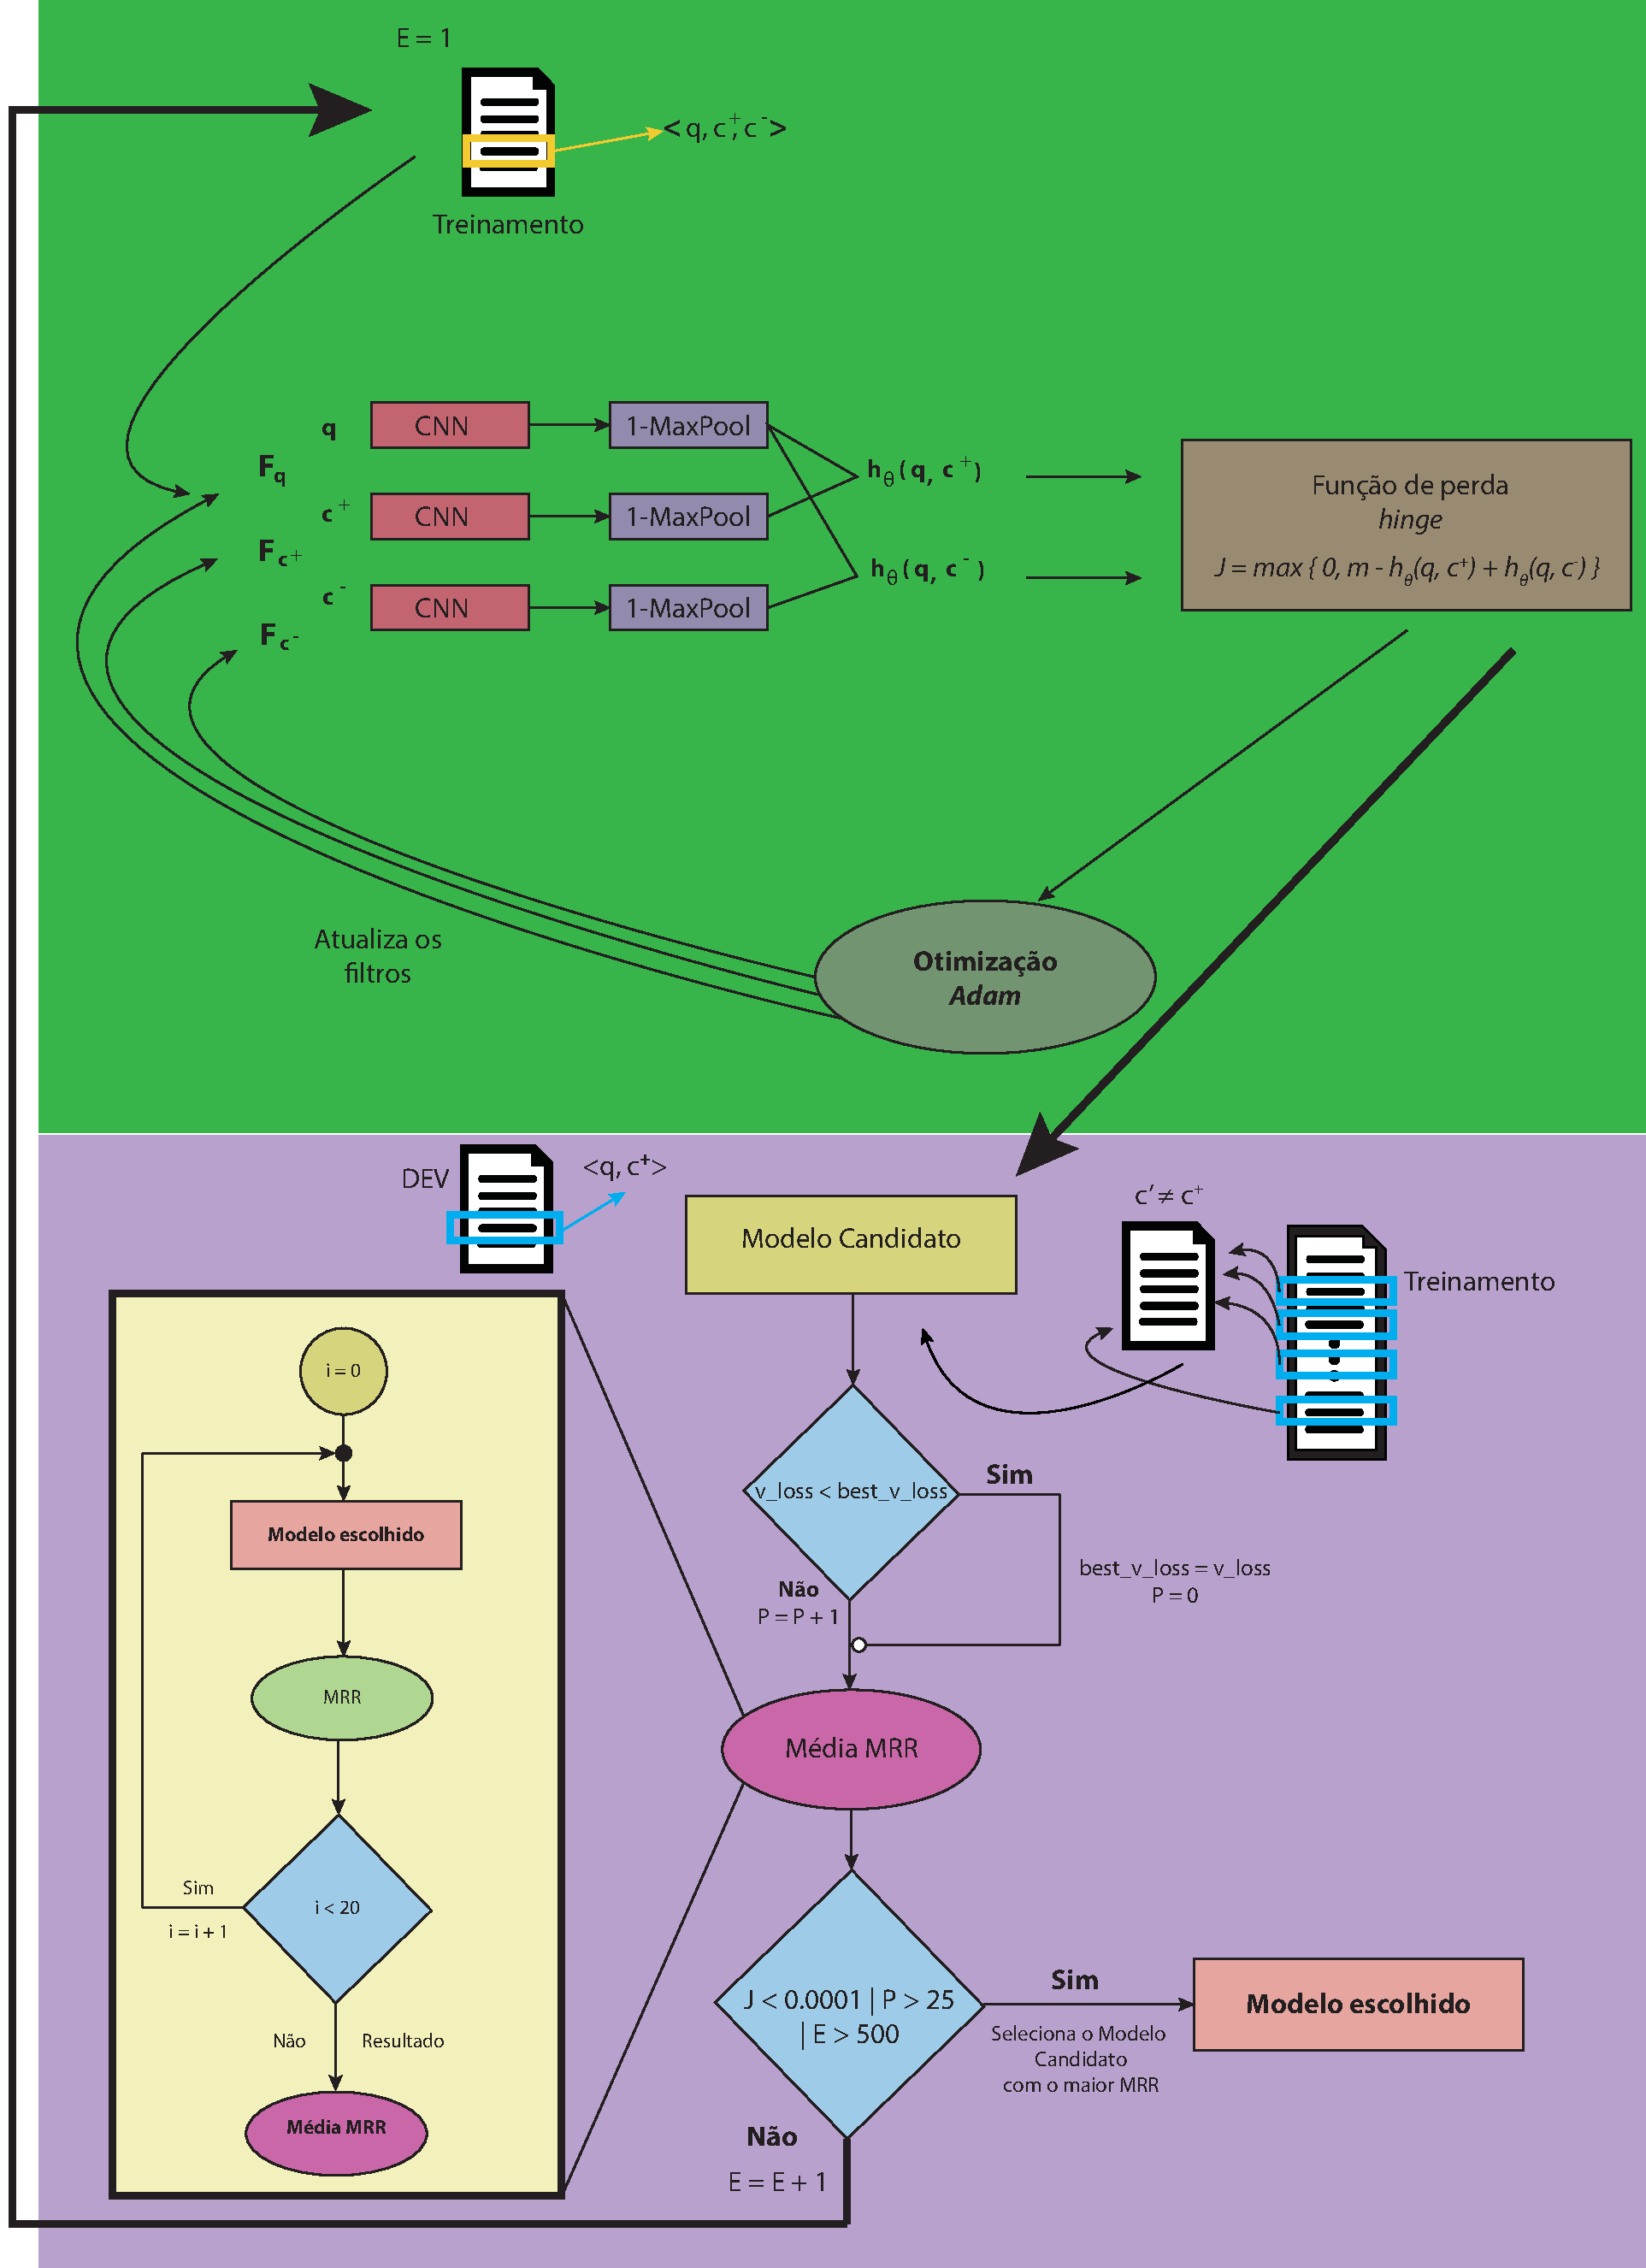
\includegraphics[height=1.5\textwidth]{figuras/cap-experimento/evaluation_process.pdf}
\caption{Boxplot.} 
\label{fig:evaluation-process}
\end{figure}

\begin{figure}[h]
\centering
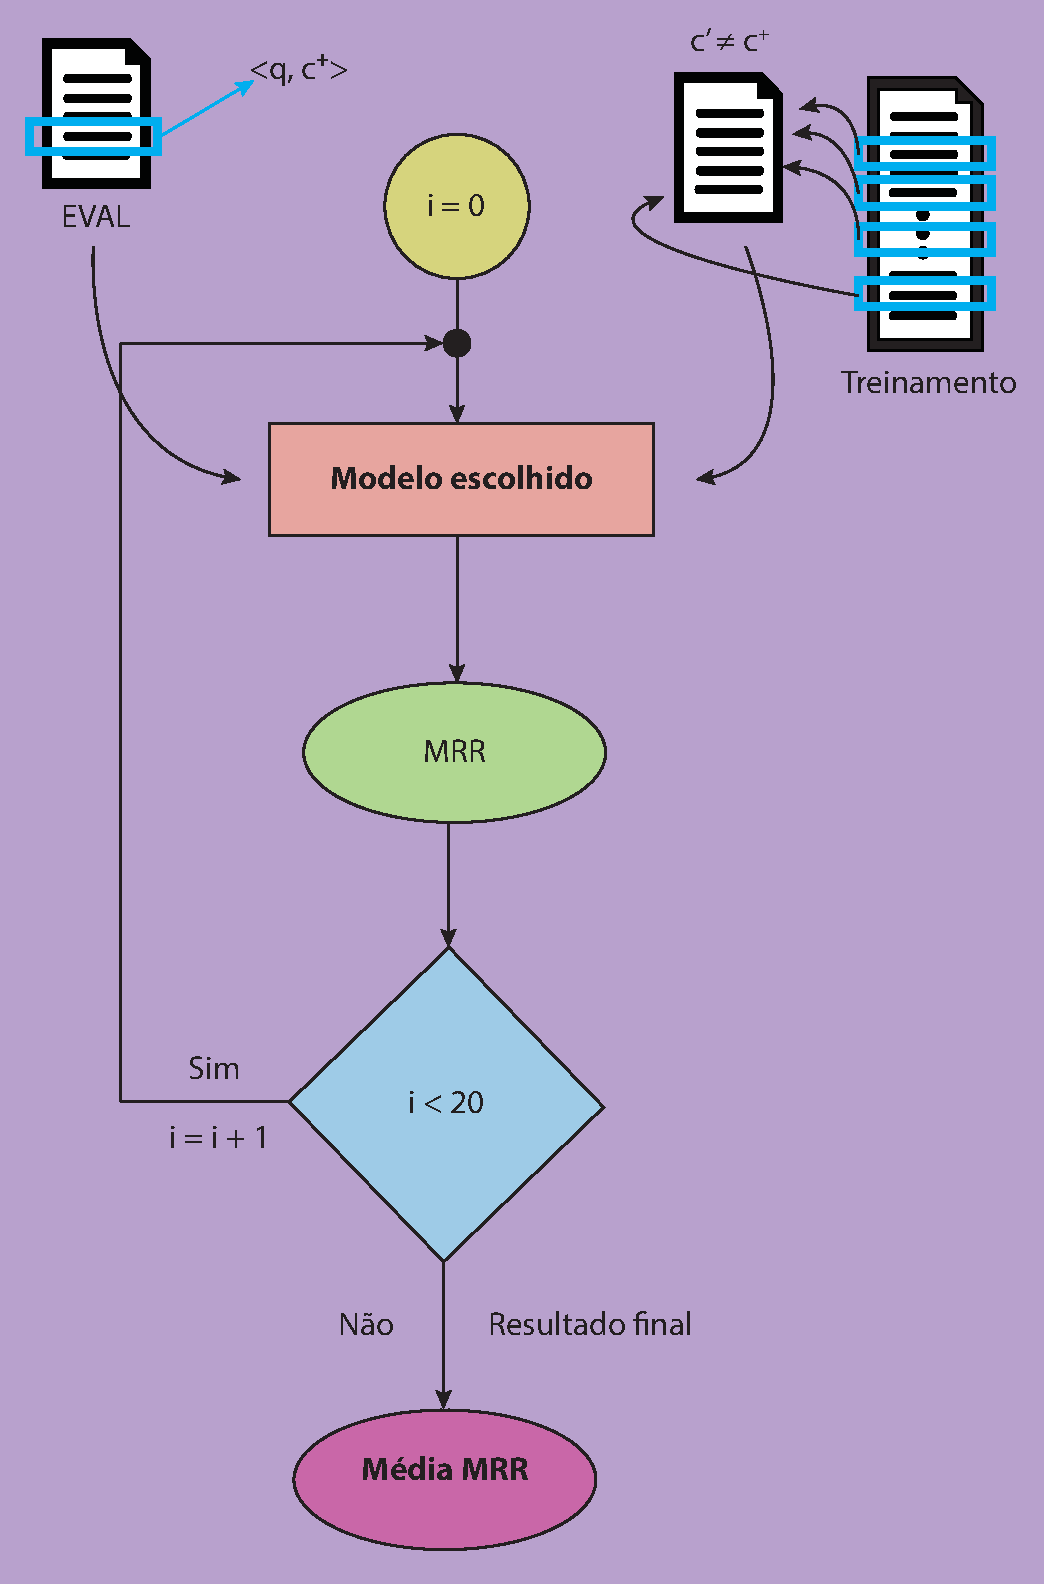
\includegraphics[height=1\textwidth]{figuras/cap-experimento/final_evaluation_process.pdf}
\caption{Boxplot.} 
\label{fig:final-evaluation-process}
\end{figure}


Durante o treinamento, do total de $60.083$ amostras, $42058$ foram utilizadas para o conjunto de treinamento e $18025$ para o conjunto de validação.

O procedimento de treinamento utilizado foi: O modelo é treinado durante 80 épocas. Caso a função de perda \textit{hinge} fique abaixo de $0,001$, o treinamento é interrompido. A cada época, o modelo é avaliado na amostra \emph{DEV}. O intuito desta avaliação é obter o melhor modelo conforme a métrica \acrshort{mrr}. Esta avaliação na amostra DEV é feita da seguinte maneira:

Para cada par $<q_{i}, c_{i}^{+}>$ da amostra \emph{DEV}, onde $q_{i}$ uma questão e $c_{i}^{+}$ uma questão anotada como correta. Outros 49 distratores $c'$ são selecionados aleatoriamente da amostra de treinamento, tal que $c_{i}^{+} \neq c'$. Para cada questão, o modelo calcula a similaridade entre a questão e os trechos de código-fonte. O cálculo de similaridade é feito através da função $h_{\theta}$, onde $h_{\theta}$ é a função \textit{cosine}. 

Posteriormente, os trechos de código-fonte são ordenados de forma decrescente, do mais similar (maior pontuação) ao menos similar (menor pontuação). Com os trechos ordenados, obtém-se a posição do trecho $c_{i}^{+}$ para cálculo do \textit{reciprocal rank}. \textit{Reciprocal rank} é o inverso da posição da primeira ocorrência de $c_{i}^{+}$ encontrada no resultado. Com o \textit{reciprocal rank}, calcula-se o \acrshort{mrr}. \acrshort{mrr} é a média do \textit{reciprocal rank} para a amostra inteira \citep{Gu-deep-code-search:2018}:

\begin{equation}
MRR = \frac{1}{n} * \sum_{i = 1}^{n}\frac{1}{p_{i}^{+}}    
\end{equation}

Onde $n$ é a quantidade de questões presentes na amostra, $p_{i}^{+}$ é a posição da primeira ocorrência do trecho $c_{i}^{+}$ entre os trechos ordenados.

Este procedimento é repetido durante 20 vezes. A cada iteração, outros 49 distratores são selecionados. Ao final, obtém-se a média \emph{MRR} do modelo. O modelo que obtiver a maior média \emph{MRR} ao final do treinamento é escolhido. A avaliação final na amostra \emph{EVAL} utiliza o mesmo procedimento da amostra \emph{DEV} descrito acima.

\section{Pré-processamento}
\label{sec:pre-processamento}

Diferente do trabalho de \cite{tan-lstm-qa}, nós geramos duas matrizes de representação distribuída distintas $\bm{T_{q}}$ e $\bm{T_{c}}$ para o vocabulário das questões e para o vocabulário dos trechos de código-fonte, conforme citado no Capítulo~\ref{cap:abordagem}. Antes de gerar a matriz $\bm{T_{c}}$, utilizamos uma função disponibilizada por \cite{yao-2018} para fazer um pré-processamento dos trechos de código-fonte. Essa função substitui os valores literais numéricos e textos pelas palavras \emph{"NUMBER"} e \emph{"STRING"}. Além disso, os comentários são removidos e as variáveis são substituídas por \emph{"VAR"}. O caractere de quebra de linha é substituído por \emph{"NEWLINE"}.

As matrizes $\bm{T_{q}}$ e $\bm{T_{c}}$ são geradas pelo \textit{word2vec} com \textit{skip-gram}. Na Figura~\ref{fig:tsne-code-snippet-python} a seguir, podemos visualizar um exemplo da representação do vetor de representação distribuída gerada pelo \textit{word2vec}. Essa imagem foi criada com o auxílio da ferramenta \textit{t-SNE}. Ela auxilia na visualização de dados de dimensão elevada \citep{scikit-learn-tsne-2019, quora-tsne-2019}. De acordo com a Figura~\ref{fig:tsne-code-snippet-python}, as palavras \emph{from} e \emph{import} são similares. Assim como \emph{if} e \emph{else}, e também \emph{list}, \emph{dict} e \emph{set}, por exemplo.

\begin{figure}[h]
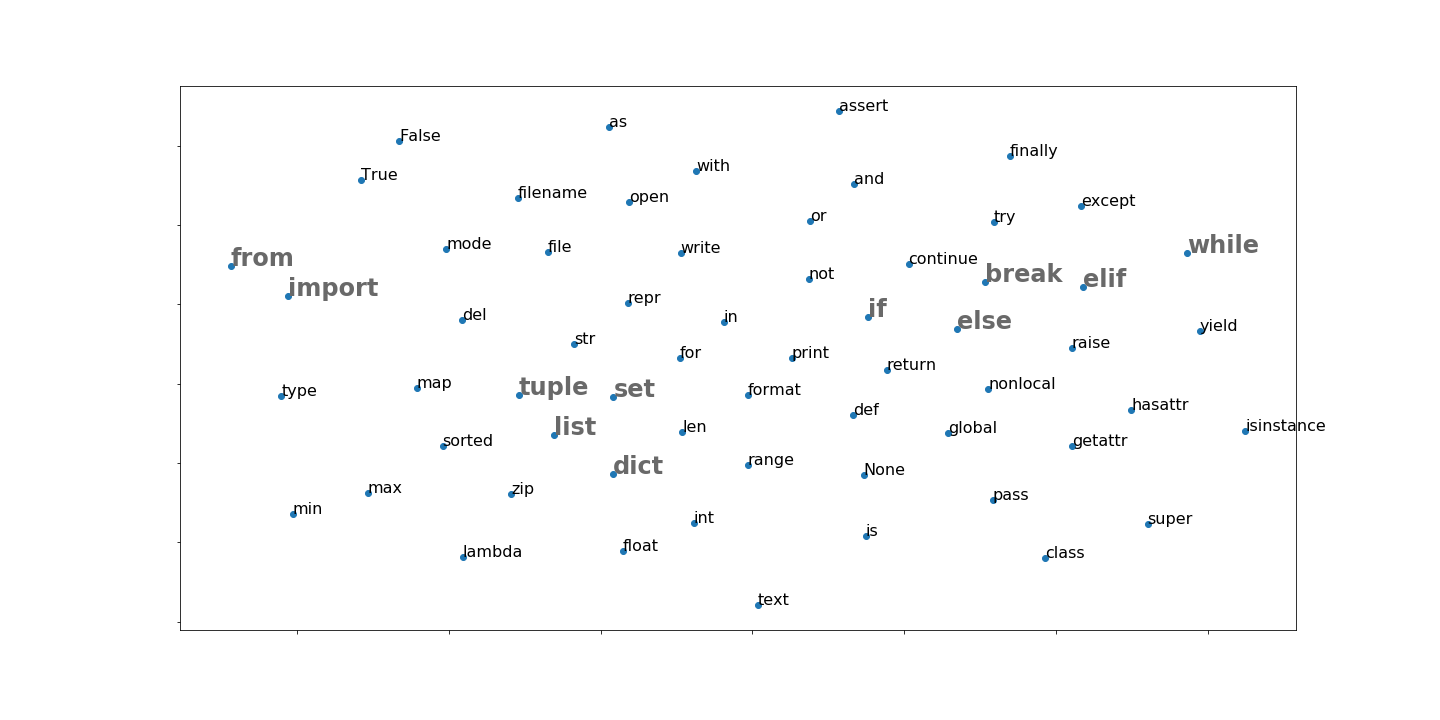
\includegraphics[width=1\textwidth]{figuras/cap-resultados-preliminares/code-tsne-output.png}
\caption{Representação em 2D do vetor de representação distribuída de trechos de código-fonte. Imagem gerada através da ferramenta t-SNE. O vetor de representação distribuída foi criado a partir da amostra de trechos de código-fonte em Python disponibilizada por \cite{yao-2018}. Vetor criado utilizando o \textit{word2vec} com o algoritmo \textit{skip-gram} e o parâmetro \textit{window} com o valor $5$.}
\label{fig:tsne-code-snippet-python}
\end{figure}

\section{Arquiteturas}

Para este estudo, comparamos a arquitetura CNN com outras duas arquiteturas: bi-LSTM com CNN e \textit{Embedding}. A arquitetura \textit{Embedding} combina os vetores de representação distribuída de cada palavra através de uma camada \textit{max pool}. A arquitetura CNN utilizada neste estudo, utiliza uma camada inicial \textit{hidden}.
Esta camada obtém um vetor $\bm{z}$ a partir das questões e trechos de código-fonte. Este vetor $\bm{z}$ servirá como entrada para a nossa arquitetura CNN que foi descrita na Seção~\ref{sec:representacao-sentenca}.

\begin{equation}
    \bm{z} = tanh(\bm{W} * \bm{x} + \bm{b})
\end{equation}

Onde $\bm{W}$ é a matriz de pesos, $\bm{x}$ é vetor que contém os vetores de representação distribuída das palavras e $\bm{b}$ é o vetor \textit{bias}. As figuras~\ref{fig:arquitetura-bi-lstm-com-cnn}, \ref{fig:arquitetura-cnn} e \ref{fig:arquitetura-embedding} ilustram as arquiteturas utilizadas:

\begin{figure}[h]
    \centering
    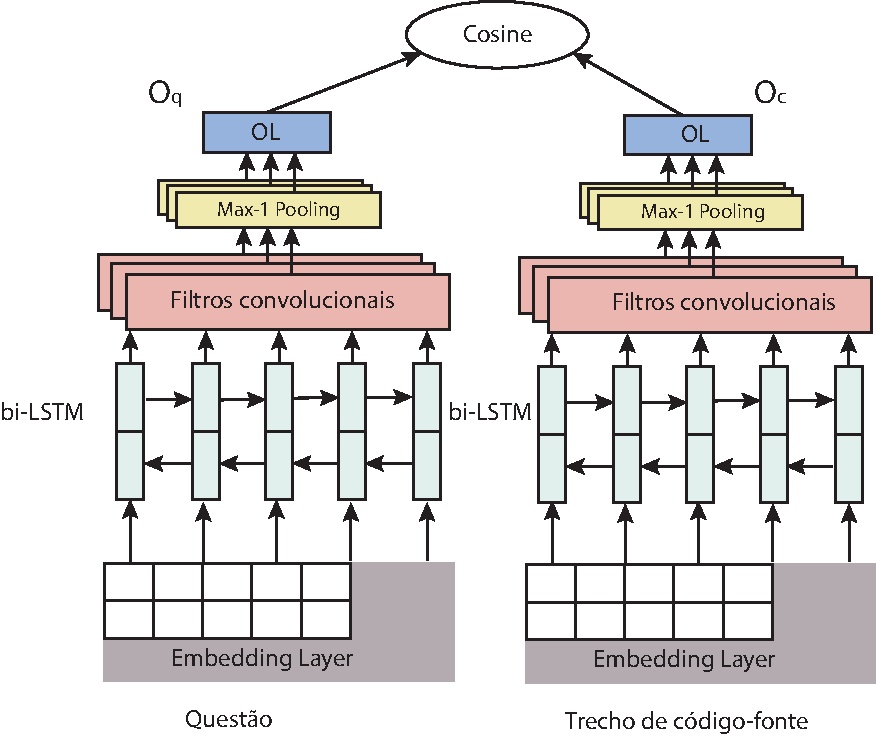
\includegraphics[width=0.6\textwidth]{figuras/cap-resultados-preliminares/ArquiteturaBiLSTM.pdf}
    \caption{Figura da arquitetura bi-LSTM com CNN. Figura utilizada no artigo \cite{marcelo-vem-2019}}
    \label{fig:arquitetura-bi-lstm-com-cnn}
\end{figure}

\begin{figure}[h]
    \centering
    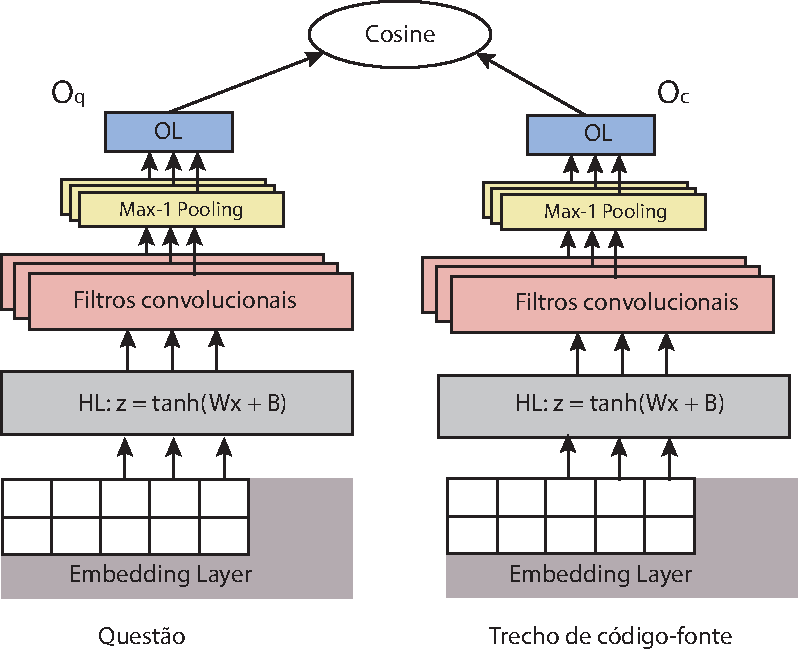
\includegraphics[width=0.6\textwidth]{figuras/cap-resultados-preliminares/ArquiteturaCNN.pdf}
    \caption{Figura da arquitetura CNN com a primeira camada de \textit{hidden layer} proposta para o artigo \cite{marcelo-vem-2019}.}
    \label{fig:arquitetura-cnn}
\end{figure}

\begin{figure}[h]
    \centering
    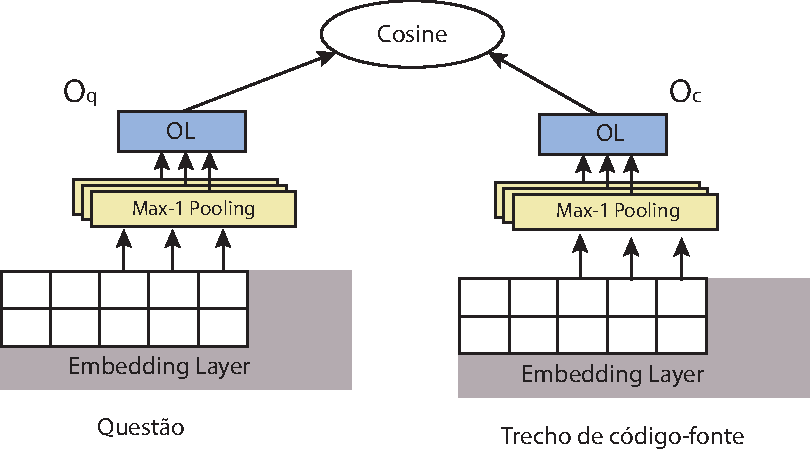
\includegraphics[width=0.6\textwidth]{figuras/cap-resultados-preliminares/ArquiteturaEmbedding.pdf}
    \caption{Figura da arquitetura de referência \textit{Embedding} para comparação. Figura utilizada no artigo \cite{marcelo-vem-2019}}
    \label{fig:arquitetura-embedding}
\end{figure}
Nas figuras \ref{fig:arquitetura-bi-lstm-com-cnn}, \ref{fig:arquitetura-cnn} e \ref{fig:arquitetura-cnn}, a palavra \textit{Embedding Layer} refere-se ao vetor de representação distribuída das palavras. \emph{OL} é um acrônimo de \textit{Output Layer} ou camada de saída. $O_{q}$ indica a camada de saída da questão. $O_{c}$ indica a camada de saída do trecho de código-fonte.

Todas as arquiteturas utilizam uma camada \textit{max pool} e, ao final, calculam a similaridade atravás da função \textit{cosine}.
Não realizamos otimização ou ajustes dos hiper-parâmetros dos modelos. Utilizamos os mesmos hiper-parâmetros propostos por \cite{tan-lstm-qa} para todas as arquiteturas. Com exceção do hiper-parâmetro filtro para a arquitetura CNN, neste caso, alteramos o valor para $100$, pois o valor $1000$ proposto por \cite{tan-lstm-qa} aumentou a capacidade do modelo e estava causando \textit{overfitting}. Para a função de perda \textit{hinge}, utilizamos o valor $0,009$ proposto por \cite{feng-2015} para a margem. Em relação a dimensão do vetor de representação distribuída das palavras (\textit{word embedding}), utilizamos o valor $100$.


%% ------------------------------------------------------------------------- %%
\section{Resultados}

Os resultados foram coletados a partir da avaliação dos modelos na amostra \emph{EVAL}. O valor final MRR é a média obtida após 20 iterações. Conforme a Tabela~\ref{table:resultados-preliminares},  a arquitetura CNN obteve um resultado próximo da arquitetura bi-LSTM com CNN. Apesar do resultado ser relativamente menor, o seu tempo de duração de treinamento é de apenas 6s, enquanto o treinamento do bi-LSTM durou cerca de 48 minutos. Tanto o treinamento quanto a avaliação foram executadas na plataforma \Gls{colab} do Google. No momento de treinamento e coleta dos resultados, a execução foi feita em uma máquina virtual com acesso a uma \acrshort{vgpu} Tesla K80.

\begin{table}[h]
\centering
\begin{tabular}{ p{10cm} P{3cm} P{3cm} }
 \hline
 \textbf{Modelos} & \textbf{Resultados MMVL (MRR)} & \textbf{Resultados MMMR (MRR)}\\
 \hline
 Embedding & $0,52 \pm 0,01$ & $0,52 \pm 0,01$\\
 
 Unif & $0,52 \pm 0,01$\\
 
 CNN - F = 50 & $0,52 \pm 0,01$\\
 
 CNN - F = 100 & $0,52 \pm 0,01$\\
 
 CNN - F = 200 & $0,52 \pm 0,01$\\
 
 CNN - F = 500 & $0,52 \pm 0,01$\\
 
 CNN - F = 1000 & $0,52 \pm 0,01$\\
 
 CNN compartilhado - F = 50 & $0,52 \pm 0,01$\\
 
 CNN compartilhado - F = 100 & $0,52 \pm 0,01$\\
 
 CNN compartilhado - F = 200 & $0,52 \pm 0,01$\\
 
 CNN compartilhado - F = 500 & $0,52 \pm 0,01$\\
 
 CNN compartilhado - F = 1000 & $0,52 \pm 0,01$\\
 
 
 \hline
 
 Unif com NL & $0,52 \pm 0,01$\\
 
 CNN com NL - F = 50 & $0,52 \pm 0,01$\\
 
 CNN com NL - F = 100 & $0,52 \pm 0,01$\\
 
 CNN com NL - F = 200 & $0,52 \pm 0,01$\\
 
 CNN com NL - F = 500 & $0,52 \pm 0,01$\\
 
 CNN com NL - F = 1000 & $0,52 \pm 0,01$\\
 
 CNN compartilhado com NL - F = 50 & $0,52 \pm 0,01$\\
 
 CNN compartilhado com NL - F = 100 & $0,52 \pm 0,01$\\
 
 CNN compartilhado com NL - F = 200 & $0,52 \pm 0,01$\\
 
 CNN compartilhado com NL - F = 500 & $0,52 \pm 0,01$\\
 
 CNN compartilhado com NL - F = 1000 & $0,52 \pm 0,01$\\
 
 \hline
\end{tabular}
\caption{Resultado preliminar do modelo CNN proposto para o artigo \cite{marcelo-vem-2019} em comparação com outras duas arquiteturas (bi-LSTM com CNN e Embedding). Estes resultados foram obtidos a partir da amostra EVAL.}
\label{table:resultados-preliminares}
\end{table}

Para entender um pouco melhor o resultado da média harmônica MRR, a figura abaixo exibe as posições da primeira ocorrência do trecho de código-fonte encontradas durante a avaliação dos modelos.

\begin{figure}[h]
    \centering
    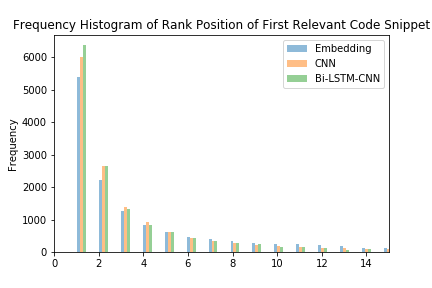
\includegraphics[width=1\textwidth]{figuras/cap-resultados-preliminares/histogram_results.png}
    \caption{Figura das primeiras posições observadas para o trecho de código-fonte anotado como correto.}
    \label{fig:histogram-mrr}
\end{figure}


Tanto o CNN quanto o bi-LSTM com CNN conseguiram classificar os trechos de código-fonte entre as 3 (três) primeiras posições em 75\% dos casos. O modelo bi-LSTM com CNN obteve uma precisão TOP-1 de 51\%, i.e., em mais da metade das vezes, o trecho de código-fonte relevante ficou na primeira posição. Já a nossa arquitetura proposta obteve um TOP-1 de aproximadamente 41\%. Um ponto a ser levantado é que a nossa métrica MRR só leva em consideração a posição apontada pelo modelo para o trecho de código-fonte anotado como correto. Mesmo que o modelo apresente um outro trecho de código-fonte que também é solução, o nosso método de avaliação não leva em consideração. Neste caso, o modelo é penalizado.

No exemplo a seguir\footnote{Este exemplo refere-se a questão \url{https://stackoverflow.com/questions/24593478/python-and-appending-items-to-text-and-excel-file}\label{foot:exemplo-resultados-preliminares}}, a rede bi-LSTM com CNN conseguiu apontar corretamente o trecho de código-fonte anotado como correto na primeira posição.
A nossa arquitetura CNN, apesar de não apresentar o trecho propriamente anotado, ele apresentou outro trecho que também serve como solução. Neste caso, apesar de ter sido penalizado, ele conseguiu responder a questão. Este é um ponto importante que teremos que analisar com cautela ao longo deste trabalho. 

\begin{tcolorbox}[colframe=orange!75!black,colback=gray!15!white,fonttitle=\bfseries,adjusted title=\large{Python and appending items to text and \colorbox{green}{excel} \colorbox{green}{file}}~\ref{foot:exemplo-resultados-preliminares},
enlarge top by=1cm%equivalent to mdframed 'skipabove'
]
\begin{mypython-without-margin}{bi-LSTM com CNN}
Yvalues = [1, 2, 3, 4, 5]
file_out = |\colorbox{green}{open}|('file.csv','wb')
mywriter=|\colorbox{green}{csv}|.|\colorbox{green}{writer}|(file_out, delimiter = '\n')
mywriter.|\colorbox{green}{writerow}|(Yvalues)
file_out.close()
\end{mypython-without-margin}

\begin{mypython-without-margin}{CNN}
import csv

with |\colorbox{green}{open}|("output.csv", "wb") as f:
    writer = |\colorbox{green}{csv}|.|\colorbox{green}{writer}|(f)
    writer.|\colorbox{green}{writerows}|(a)
\end{mypython-without-margin}

\end{tcolorbox}

\subsection{Ameaças à validade}

Conforme citado anteriormente, \cite{yao-2018} anotaram o conjunto de dados utilizando um framework proposto em seu artigo. Para anotá-los, os autores treinaram uma rede neural no conjunto de dados anotado manualmente. Em nosso trabalho, fizemos o caminho inverso. Treinamos os nossos modelos nos dados anotados automaticamente e avaliamos no conjunto anotado manualmente. Para diminuir o viés, adotamos o procedimento proposto por \cite{iyer-etal-2016-summarizing} descrito na Seção~\ref{sec:treinamento-avaliacao}.

\subsection{Considerações}

Os resultados apresentados pelo nosso modelo CNN parecem bastante promissores, a nosso ver. O próximo passo é comparar o nosso modelo com o modelo proposto por \cite{cambronero-deep-learning-code-search:2019}, que é o estado da arte. 

Não fizemos ajustes dos hiper-parâmetros e nem uso de regularização durante o treinamento. Na Figura \ref{fig:grafico-erro-cnn} abaixo, podemos ver que o CNN apresenta uma diferença grande entre a curva de erro na amostra de validação e da amostra de treinamento, principalmente a partir da época $5$ (eixo $X$), próximo da interrupção do treinamento. Isto é um indicativo de \textit{overfitting}. A arquitetura bi-LSTM com CNN apresenta o mesmo problema (ver Figura~\ref{fig:grafico-erro-bi-lstm-cnn}). Já no caso da arquitetura \textit{Embedding}, Figura \ref{fig:grafico-embedding}, as duas curvas de erro estão próximas até a interrupção. 

\begin{figure}[h]
    \centering
    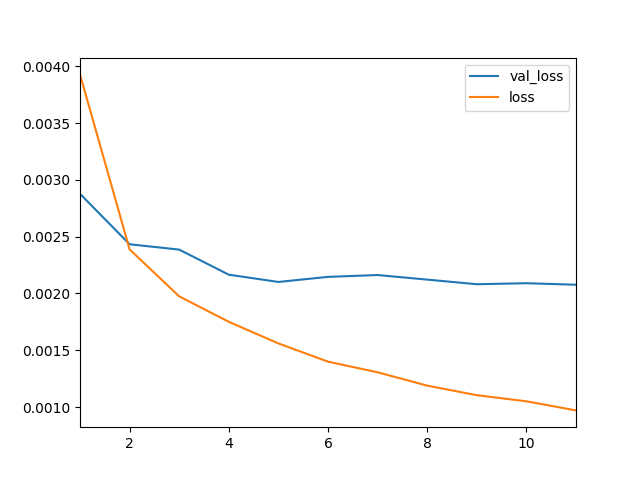
\includegraphics[width=1\textwidth]{figuras/cap-resultados-preliminares/569229_ConvolutionalLSTM_plot.png}
    \caption{Gráfico do treinamento do modelo bi-LSTM com CNN. Gráfico do erro de validação (\emph{val\_loss}) e erro na amostra de treinamento (\emph{loss}) por época (\emph{eixo X}). O melhor modelo em relação a métrica MRR foi obtido na época $9$.}
    \label{fig:grafico-erro-bi-lstm-cnn}
\end{figure}

\begin{figure}[h]
    \centering
    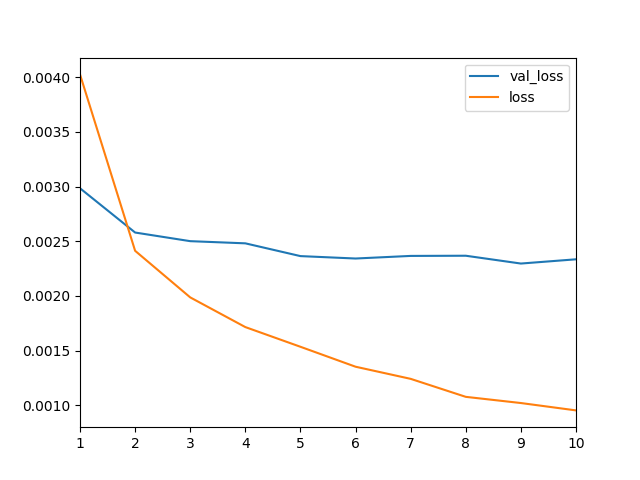
\includegraphics[width=1\textwidth]{figuras/cap-resultados-preliminares/569229_ConvolutionModel_plot.png}
    \caption{Gráfico do treinamento do CNN. Gráfico do erro de validação (\emph{val\_loss}) e erro na amostra de treinamento (\emph{loss}) por época (\emph{eixo X}). O melhor modelo em relação a métrica MRR foi obtido na época $9$.}
    \label{fig:grafico-erro-cnn}
\end{figure}

\begin{figure}[h]
    \centering
    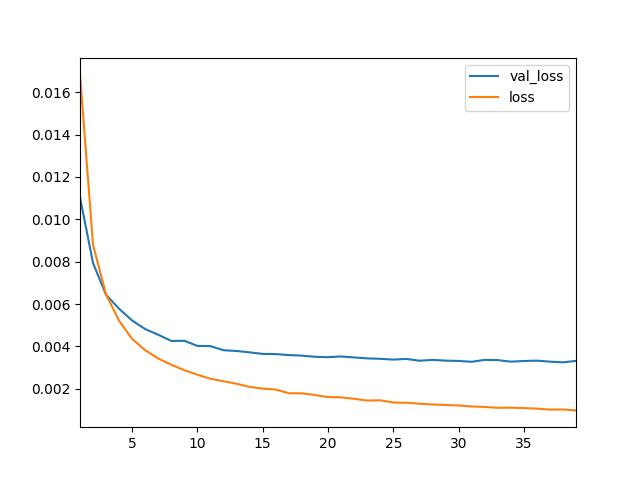
\includegraphics[width=1\textwidth]{figuras/cap-resultados-preliminares/569229_EmbeddingModel_plot.png}
    \caption{Gráfico do treinamento do modelo \textit{Embedding}. Gráfico do erro de validação (\emph{val\_loss}) e erro na amostra de treinamento (\emph{loss}) por época (\emph{eixo X}). O melhor modelo em relação a métrica MRR foi obtido na época $39$.}
    \label{fig:grafico-embedding}
\end{figure}

Podemos perceber que de acordo com as figuras~\ref{fig:grafico-erro-cnn} e \ref{fig:grafico-erro-bi-lstm-cnn}, tanto o CNN quanto o bi-LSTM com CNN tem uma margem a melhorar. Além da margem de melhora no treinamento, uma análise mais detalhada do resultado é necessária. Conforme o exemplo citado na seção anterior, o modelo CNN apresentou uma resposta correta para a pergunta, porém foi penalizada pois não era exatamente o trecho anotado como correto. Caso haja mais casos deste tipo, podemos adotar o mesmo procedimento proposto por \cite{cambronero-deep-learning-code-search:2019} de avaliação automática. Um trecho será considerado correto quando a diferença do resultado da função $h_{\theta}$ de similaridade entre ele e o trecho anotado como correto estiver dentro de um certo intervalo.
